% !TEX TS-program = lualatex
\documentclass{standalone}
\usepackage{tikz, pgfplots}
\pgfplotsset{compat=1.18}
\begin{document}
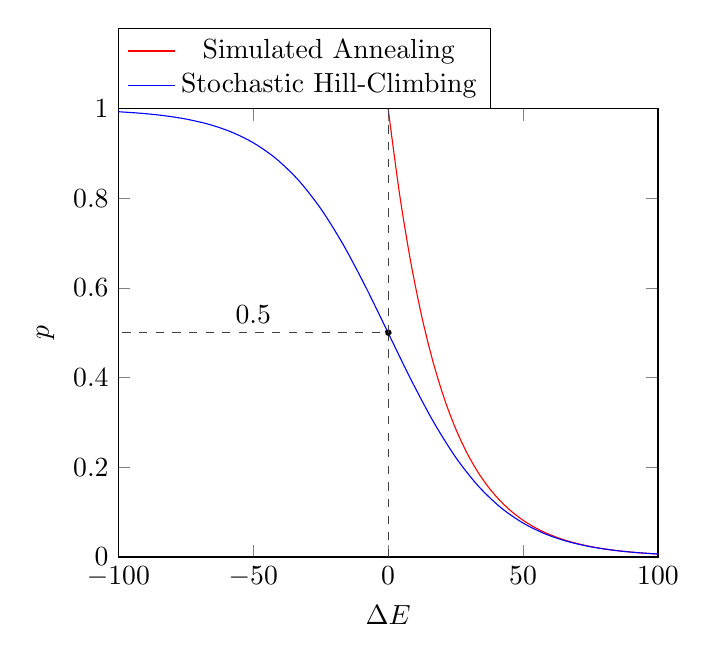
\begin{tikzpicture}
    \begin{axis}[
        xlabel=$\Delta E$,
        ylabel=$p$,
        ymin=0, ymax=1,
        xmin=-100,xmax=100,
        legend style={at={(axis description cs:0,1)}, anchor=south west}
    ]
        \addplot[smooth, domain=0:100,red]{exp(-x/20)};
        \addplot[smooth, domain=-100:100,blue]{1/(1+exp(x/20))};
        \draw[dashed,darkgray](0,0)--(0,0.5)node[draw,circle,black, fill=black, inner sep=0.75pt]{}--(-100,0.5)node[black,midway, above]{$0.5$};
        \draw[dashed,darkgray](0,0.5)--(0,1);
    \legend{Simulated Annealing, Stochastic Hill-Climbing};
    \end{axis}
\end{tikzpicture}
\end{document}